\section{Расширение изначально однородно заряженного шара}

\textit{Первый метод}. 

Рассмотрим эту задачу с точки зрения симметрии. Во-первых, понятно, что в системе отсутствует магнитное поле. Во-вторых, плотность заряда $\rho$ и поле скоростей $\vec{v}$ зависят только от расстояния до центра шара. Также скорость имеет только одну компоненту $v_r$, также как и электрическое поле $E_r$.
 
Выберем внутри шара радиуса $R$ заряд которой равен $Q$ сферу радиуса $r_0$. Такая сфера ограничивает заряд:
\[
	q = \frac{r_0^3}{R^3} Q
\]

Найдём как движется точка на поверхности такой сферы. Уравнение движения:
\[
	\frac{d^2 r}{dt^2} = A E_r = A  k \frac{q}{r^2}
\]
\[
	\frac{v_r^2}{2} - \frac{v_{0r}^2}{2} = A k q \left(- \frac{1}{r} + \frac{1}{r_0}\right)
\]
\[
	v_r = \sqrt{v_{0r}^2 + \frac{2A kq}{r_0} - \frac{2A k q}{r}} = \sqrt{a - \frac{b}{r}}
\]
\[
	\int\limits_{r_0}^{r} 
	\frac{\sqrt{r} dr}{\sqrt{ar - b}}
	=
	t - t_0
\]
\[
	\frac{b}{a^{3/2}} 
	\left.
	\left(\sqrt{\frac{ar}{b}} \sqrt{\frac{ar}{b}-1} + 
	\ln \left|\sqrt{\frac{ar}{b} - 1} + \sqrt{\frac{ar}{b}}\right|\right) 
	\right|_{r_0}^{r}
	= t - t_0
\]
В случае если $v_{r}(0) = 0$, получаем:
\[
	b = 2A k q
\]
\[
	a = \frac{2A kq}{r_0}
\]
\[
	\frac{r_0^{3/2}}{(2A k q)^{1/2}} 
	\left(\sqrt{\frac{r}{r_0}} \sqrt{\frac{r}{r_0}-1} + 
	\ln \left|\sqrt{\frac{r}{r_0} - 1} + \sqrt{\frac{r}{r_0}}\right|\right)
	= t
\]
\[
	\left(\sqrt{\frac{r}{r_0}} \sqrt{\frac{r}{r_0}-1} + 
	\ln \left|\sqrt{\frac{r}{r_0} - 1} + \sqrt{\frac{r}{r_0}}\right|\right)
	= \sqrt{
		\frac{2A k Q}{R^{3}} } t = f\left(\frac{r}{r_0}\right)
\]
На рисунке приведена зависимость $r(t)$, для различных значений $r_0$.
\begin{figure}[h!]
	\centering
	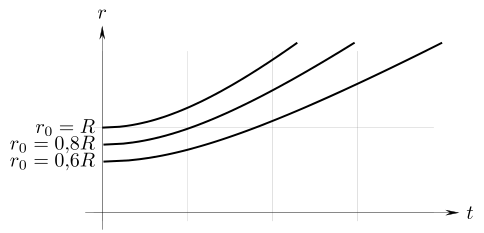
\includegraphics[width=0.5\textwidth]{images/png/sphere1.png}
\end{figure}
\\
Плотность зарядов можно найти, определяя для каждого из слоёв, между которыми находится заряд $dq$, толщина между слоями $dr_0$, в момент времени $t$ соответствующее расстояние между слоями:
$dr$:
\[
\rho = \frac{1}{4\pi r^2} \frac{dq}{dr},
\]
где $dr$ определяется $dr_0$, а $dt = 0$. В результате:
\[
	f'\left(\frac{r}{r_0}\right) \frac{dr}{r_0} = f'\left(\frac{r}{r_0}\right) \frac{r dr_0}{r_0^2} 
\]
\[
	\frac{dr}{r} = \frac{dr_0}{r_0}
\]
\[
	\rho = \frac{Q}{4\pi R^3/3} \left(\frac{r_0}{r}\right)^3 = \rho_0 \left(f^{-1}\left(\sqrt{
		\frac{2\alpha k Q}{R^{3}} } t\right)\right)^{-3}
\]
То есть $\rho$ зависит только от времени и не зависит от расстояния, что означает, что шар всегда однороден.

\textit{Второй метод}.

С точки зрения уравнений Максвелла в сферически-симметричном случае:
\[
	\begin{aligned}
		& \begin{vmatrix}
			\cfrac{1}{r^2 \sin \theta} \,\vec{e}_r & \cfrac{1}{r \sin \theta}\, \vec{e}_\theta & \cfrac{1}{r} \, \vec{e}_\alpha \\
			\df{r} & 0 & 0 \\
			E_r & r E_\theta & r \sin \theta E_\alpha
		\end{vmatrix}
		= 
		- \dff{\vec{B}}{t} \\
		& \begin{vmatrix}
		\cfrac{1}{r^2 \sin \theta} \,\vec{e}_r & \cfrac{1}{r \sin \theta}\, \vec{e}_\theta & \cfrac{1}{r} \, \vec{e}_\alpha \\
		\df{r} & 0 & 0 \\
		B_r & r B_\theta & r \sin \theta B_\alpha
		\end{vmatrix}
		= 
		\mu_0 \rho \vec{v} + \frac{1}{c^2} \dff{\vec{E}}{t} \\
		& \frac{1}{r^2} \df{r} \left( r^2 E_r\right) = \frac{\rho}{\varepsilon_0} \\ 
		& \frac{1}{r^2} \df{r} \left( r^2 B_r\right) = 0 \\
		& \left(\dff{\vec{v}}{t} + \vec{v}\cdot\nabla\vec{v}\right) = A \left(\vec{E} + 
		\begin{vmatrix}
		\vec{e}_r & \vec{e}_\theta & \vec{e}_\alpha \\
		v_r & v_\theta & v_\alpha \\
		B_r & B_\theta & B_\alpha
		\end{vmatrix} \right)
	\end{aligned}
	\Rightarrow
	\begin{aligned}
		& \dff{B_r}{t} = 0 \\
		& \dff{B_\theta}{t} = \frac{1}{r} \df{r} \left( r E_\alpha\right) \\
		& \dff{B_\alpha}{t} = - \frac{1}{r} \df{r} \left( r E_\theta\right) \\
		& \dff{E_r}{t} = - \frac{\rho v_r}{\varepsilon_0} \\
		& \dff{E_\theta}{t} = - c^2 \frac{1}{r} \df{r} \left( r B_\alpha\right) - \frac{\rho v_\theta}{\varepsilon_0} \\
		& \dff{E_\alpha}{t} = c^2\frac{1}{r} \df{r} \left( r B_\theta\right) - \frac{\rho v_\alpha}{\varepsilon_0}\\
		& \frac{1}{r^2} \df{r} \left( r^2 E_r\right) = \frac{\rho}{\varepsilon_0} \\ 
		& \frac{1}{r^2} \df{r} \left( r^2 B_r\right) = 0 \\
		& \dff{v_r}{t} = - v_r\dff{v_r}{r} + A\left(E_r + v_\theta B_\alpha - v_\alpha B_\theta\right) \\
		& \dff{v_\theta}{t} = - v_r\dff{v_\theta}{r} + A\left(E_\theta + v_\alpha B_r - v_r B_\alpha\right) \\
		& \dff{v_\alpha}{t} = - v_r\dff{v_\alpha}{r} + A\left(E_\alpha + v_r B_\theta - v_\theta B_r\right) \\
	\end{aligned}
\] 
Если в начальный момент времени:
\[
	E_\alpha, E_\theta, B_r, B_\alpha, B_\theta, v_\theta, v_\alpha, v_r = 0,
\]
то как следует из системы уравнений первого порядка по времени, во все следующие моменты времени:
\[
	E_\alpha, E_\theta, B_r, B_\alpha, B_\theta, v_\theta, v_\alpha = 0,
\]
Остаётся система из трёх уравнений:
\[
	\begin{aligned}
	& \dff{E_r}{t} = - \frac{\rho v_r}{\varepsilon_0} \\
	& \frac{1}{r^2} \df{r} \left( r^2 E_r\right) = \frac{\rho}{\varepsilon_0} \\
	& \dff{v_r}{t} = - v_r\dff{v_r}{r} + A E_r
	\end{aligned}
\]
Отсюда легко получить систему:
\[
	\begin{aligned}
	& \dff{r^2 E_r}{t} + v_r \df{r} \left( r^2 E_r\right) = 0 \\
	& \dff{v_r}{t} + v_r\dff{v_r}{r} = A E_r
	\end{aligned}
\]
Как её решать? Методом характеристик. Все уравнения имеют один и тот же вид и представляют собой уравнения переноса. Скорость переноса $v_r$. Система в методе характеристик:
\[
	\begin{aligned}
	& \Dff{r}{t} = v_r \\
	& \Dff{(r^2 E_r)}{t} = 0 \\
	& \Dff{v_r}{t} = A E_r
	\end{aligned}
\]
Из второго уравнения следует, что:
\[
	E_r = \frac{E_r(0) r_0^2}{r^2} = k\frac{r_0^3}{R^3 r^2} Q = k \frac{q}{r^2}
\]
И система сводится к системе из предыдущего метода.

\section{Влияние гравитации поля на заряженный шар}

Поле имеет энергию и следовательно массу. Резонно предположить, что эта масса должна участвовать в гравитационных взаимодействиях и гравитация поля должна влиять на движение заряженной среды. Попробуем это учесть.

В сферически симметричном случае массу поля, ограниченная сферой радиуса $r(r_0, t)$, можно найти из выражения:
\[
	m = \frac{\varepsilon_0}{2c^2} \int\limits_0^{r(r_0, t)} E_r^2 4 \pi r^2 dr = 
	\frac{4\pi k^2 \varepsilon_0 Q^2}{2c^2 R^6} \int\limits_0^{r_0} \frac{r_0^6}{r^2} \dff{r}{r_0} dr_0 =
	\frac{k Q^2}{2c^2 R^6} \int\limits_0^{r_0} \frac{r_0^6}{r^2} \dff{r}{r_0} dr_0
\]

Будем считать, что гравитация Ньютонова, случай нерелятивистский, плотность заряда и плотность массы пропорциональны:
\[
	\alpha \rho = \rho_m
\]
Тогда получим уравнения движения:
\[
	\Dff{v_r}{t} = (A + G \alpha / k) k\frac{r_0^3}{R^3 r^2} Q + \frac{k Q^2}{2c^2 R^6} \int\limits_0^{r_0} \frac{r_0^6}{r^2} \dff{r}{r_0} dr_0
\]


\section{Метод характеристик для уравнений Максвелла}

Метод характеристик удобно применять для среды, описываемой уравнениями гидродинамики. Система уравнений Максвелла и второй закон Ньютона для заряженной жидкости с отношением заряда к массе для частицы среды $A$:
\[
	\begin{aligned}
	& \div \vec{E} = \frac{\rho}{\varepsilon_0} \\
	& \rot \vec{E} = - \dff{\vec{B}}{t}\\
	& \div \vec{B} = 0 \\
	& \rot \vec{B} = \mu_0 \rho \vec{v} + \frac{1}{c^2} \dff{E}{t} \\
	& \dff{\vec{v}}{t} + (\vec{v}\cdot\nabla) \vec{v} = \vec{a}(A(\vec{E} + \vec{v}\times\vec{B}))
	\end{aligned}
	\Rightarrow
	\begin{aligned}
	& \Dff{\vec{E}}{t} = c^2 \rot \vec{B} - \vec{v} \div \vec{E} + (\vec{v} \cdot \nabla) \vec{E} \\
	& \Dff{\vec{B}}{t} = - \rot \vec{E} + (\vec{v} \cdot \nabla) \vec{B} \\
	& \Dff{\vec{v}}{t} = \vec{a}(A(\vec{E} + \vec{v}\times\vec{B})) \\
	& \Dff{\vec{r}}{t} = \vec{v}
	\end{aligned}
\] 
\[
	\begin{aligned}
	& \Dff{\vec{E}}{t} = c^2 \nabla_B \times \vec{B} - \vec{v} (\nabla_E \cdot \vec{E}) + (\vec{v} \cdot \nabla_E) \vec{E} =
		c^2 \nabla_B \times \vec{B} - \nabla_E \times (\vec{v} \times \vec{E}) =
		c^2 \nabla_{E, B} \times \left(\vec{B} - \frac{\vec{v}}{c^2} \times \vec{E}\right) \\
	& \Dff{\vec{B}}{t} = -  \nabla_E \times \vec{E} - \vec{v} (\nabla_B \cdot \vec{B}) + (\vec{v} \cdot \nabla_B) \vec{B} =
		- \nabla_E \times \vec{E} - \nabla_B \times (\vec{v} \times \vec{B}) =
		- \nabla_{E, B} \times \left(\vec{E} + \vec{v} \times \vec{B}\right) \\
	& \Dff{\vec{v}}{t} = \vec{a}(A(\vec{E} + \vec{v}\times\vec{B})) \\
	& \Dff{\vec{r}}{t} = \vec{v}
	\end{aligned}
\]
Последняя система интересна тем, что вскрывает некоторые внутренние связи, но предыдущая система лучше поддаётся анализу. Итак,
\[
	\begin{aligned}
	& \Dff{\vec{E}}{t} = c^2 \rot \vec{B} - \vec{v} \div \vec{E} + (\vec{v} \cdot \nabla) \vec{E} \\
	& \Dff{\vec{B}}{t} = - \rot \vec{E} + (\vec{v} \cdot \nabla) \vec{B} \\
	& \Dff{\vec{v}}{t} = \vec{a}(A(\vec{E} + \vec{v}\times\vec{B})) \\
	& \Dff{\vec{r}}{t} = \vec{v}
	\end{aligned}
\]
Начальные условия:
\[
	\vec{E}(\vec{r}_0, t_0), \quad \vec{B}(\vec{r}_0, t_0),  \quad\vec{v}(\vec{r}_0, t_0), \quad \vec{r}(t_0) = \vec{r}_0
\]
Решением системы будут выражения:
\[
	\vec{E}(\vec{r}_0, t), \quad \vec{B}(\vec{r}_0, t),  \quad\vec{v}(\vec{r}_0, t), \quad \vec{r}(\vec{r}_0, t)
\]
Здесь $\vec{r}_0$ аналог постоянной интегрирования. Первые три выражения показывают как меняется электромагнитные поля и поле скоростей в различные моменты времени вдоль характеристики. Выбирая в качестве $\vec{r}_0$ все точки пространства, можно получить поле во всём пространстве в различные моменты времени.